% Provenance (never printed): old seconde/premiere S material on the water
% cycle on land (the drainage basin, river discharge, floods and their
% management); see sources/book2/PROVENANCE.md. The Varden basin is computed
% in figdata/grade-10/varden_basin.py from figdata/shared/region.py; the
% Potomac record in figdata/grade-10/flood_frequency.py.
\chapter{अपवाह द्रोणियाँ, नदियाँ और बाढ़}\label{ch:g10:drainage-basins}

वर्षा रुकने के दो दिन बाद कोई नदी ऐसे नगर में चढ़ सकती है जहाँ ज़रा भी
वर्षा नहीं हुई। जो जल उसकी गलियों में भर जाता है, वह पहले गिरा था, बहुत ऊपर की ओर की
पहाड़ियों पर; वह उनकी ढलानों से बहकर नालों में गया, और नाले मिलकर
उस नदी में बदल गए जो उसे एक साथ नगर तक ले आई। किसी बाढ़ को समझने के लिए
नदी से आगे उस पूरे क्षेत्र को देखना पड़ता है जो उसे पोषित करता है, और
उसमें से होकर जल का अनुसरण करना पड़ता है। यह अध्याय उस क्षेत्र, \omterm{def:g10:drainage-basins:drainage-basin}{अपवाह
द्रोणी}, की परिभाषा देता है; मापता है कि नदी कितना ले जाती है, यानी उसका \omterm{def:g10:drainage-basins:discharge}{विसर्जन}; नदी के
किसी बिंदु से गुज़रती बाढ़ का अनुसरण करता है; और दिखाता है कि बाढ़ों का एक लंबा अभिलेख कैसे बताता है कि
कोई दी हुई बाढ़ कितनी बार लौटकर आती है।

\begin{omfigure}
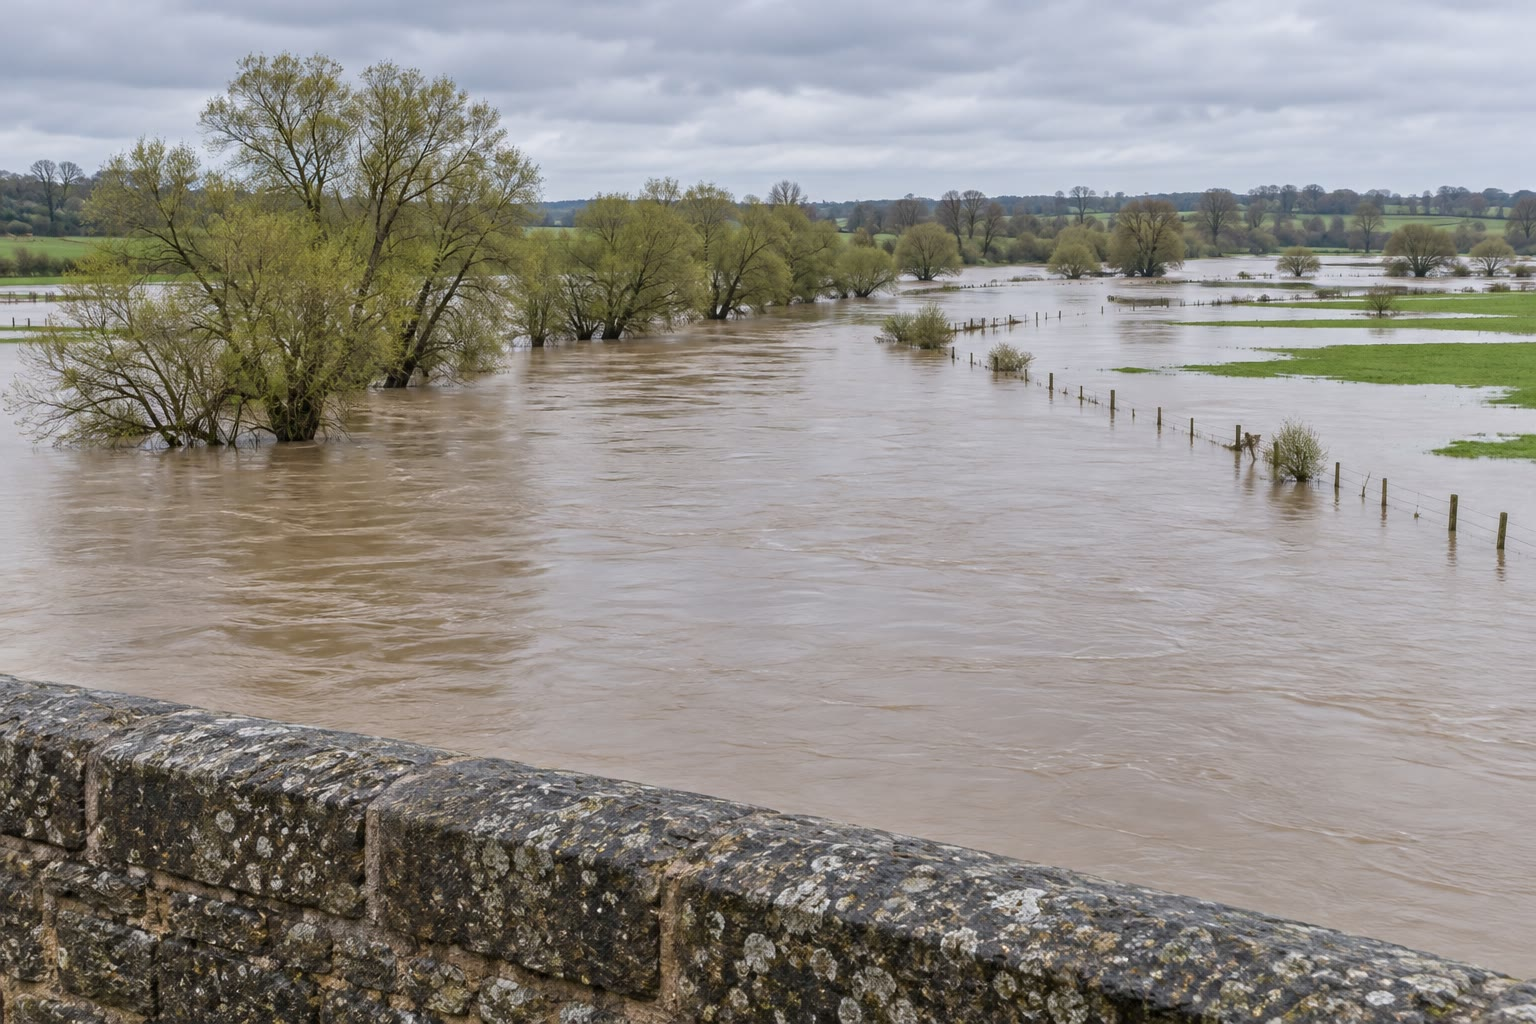
\includegraphics[width=0.8\linewidth]{images/book2/ai/g10-river-flood-meadows.jpg}

{\small पत्थर के एक पुल से दिखती बाढ़ में एक नदी: कीचड़ से लदा भूरा जल
अपनी धारा से बाहर निकलकर अपने बाढ़ के मैदान की चरागाहों को ढक चुका है, उन बाड़ों
और पेड़ों तक जो उसके सामान्य किनारों पर कतार में खड़े हैं।}
\end{omfigure}

\begin{recall}
ज़मीन तक पहुँचने वाली वर्षा उसमें रिस जाती है, उसकी सतह पर बह जाती है, या
वाष्पित हो जाती है; जल चक्र उसे वापस समुद्र तक ले जाता है (भौतिकी की पुस्तकें)। जल पारगम्य चट्टानों में रिसकर
भौम जलस्तर के नीचे उन्हें भर देता है, और जलभृत बनाता है जो सोतों और नदियों को पोषित करते हैं (पुस्तक 1,
कक्षा 6)। नदी अपने समतल बाढ़ के मैदान में विसर्पों में घूमती हुई बहती है, जिसे वह
बाढ़ के समय ढक देती है (पुस्तक 1, कक्षा 5)। समोच्च रेखाएँ समान
ऊँचाई के बिंदुओं को जोड़ती हैं; वार्डन पहाड़ियाँ इस शृंखला के मानचित्रों पर बना क्षेत्र हैं
(पुस्तक 1, कक्षा 2 और 9)।
\end{recall}

\begin{safety}
बाढ़ का जल जितना दिखता है उससे कहीं अधिक ख़तरनाक होता है। तेज़ बहते जल के लगभग \qty{15}{cm}
किसी वयस्क को गिरा सकते हैं, और लगभग \qty{30}{cm} किसी
कार को बहा ले जा सकते हैं; उसके नीचे की सड़क धँस चुकी हो सकती है। बाढ़ के जल में कभी पैदल न
जाइए और न गाड़ी चलाइए: मुड़ जाइए और दूसरे रास्ते से जाइए।
% ledger: nws:flood-water
\end{safety}

\section{अपवाह द्रोणी}

वर्षा की हर बूँद जो वाष्पित नहीं होती या गहराई तक नहीं रिसती, ढलान पर नीचे बहती है।
वह ज़मीन की सबसे तीव्र ढलान का अनुसरण करती है, किसी क्षुद्र-सरिता में मिलती है, फिर किसी नाले में,
और नाले मिलकर नदियाँ बनते हैं। वह सारी भूमि जिसका जल एक ही
नदी में पहुँचता है, एक इकाई बनाती है।

\begin{definition}[अपवाह द्रोणी; जल-विभाजक]\label{def:g10:drainage-basins:drainage-basin}
नदी के किसी बिंदु की \emph{अपवाह द्रोणी}\index{अपवाह द्रोणी}
भूमि का वह पूरा क्षेत्र है जिसका अपवाह उस बिंदु से ऊपर की ओर नदी में बहता है और
उस बिंदु से गुज़रता है।
\emph{जल-विभाजक}\index{जल-विभाजक} वह रेखा है जो दो पड़ोसी अपवाह द्रोणियों को अलग करती है: वह
भूमि के शिखरों का अनुसरण करती है, और उसके दोनों ओर गिरने वाली वर्षा
अलग-अलग नदियों में बहती है।
\end{definition}

द्रोणी की परिभाषा हमेशा नदी के किसी बिंदु के लिए होती है, जो उसका \emph{निकास} है:
समुद्र तक पहुँचने के स्थान पर नदी की द्रोणी सबसे बड़ी होती है, और ऊपर की ओर का हर बिंदु
उसके भीतर एक छोटी द्रोणी रखता है। किसी \omterm{def:g10:drainage-basins:drainage-basin}{जल-विभाजक} के दोनों ओर एक मीटर की दूरी पर
गिरने वाली दो बूँदें अलग-अलग नदियों में, और अलग-अलग
महासागरों में भी, पहुँच सकती हैं।

\subsection*{वार्डन नदी की द्रोणी}

कंप्यूटर ऊँचाइयों के मानचित्र से कुछ चरणों में \omterm{def:g10:drainage-basins:drainage-basin}{अपवाह द्रोणी} ज्ञात करता है।
मानचित्र को छोटे वर्गों में काटा जाता है, यहाँ हर एक की भुजा \qty{50}{m} है। हर वर्ग के लिए
कंप्यूटर उसके आठ पड़ोसियों को देखता है और जल को उस पड़ोसी की ओर भेजता है
जहाँ सबसे तीव्र नीचे की ढलान से पहुँचा जाता है। (जहाँ किसी छोटे गड्ढे का कोई निचला
पड़ोसी नहीं होता, उसे पहले उस तल तक भर दिया जाता है जिस पर वह छलक पड़े, जैसे
कोई पोखर छलकता है।) वर्ग से वर्ग तक इन चरणों का अनुसरण करने से मानचित्र पर कहीं से भी
किसी बूँद का मार्ग बन जाता है। जिन वर्गों की बूँदें नदी तक पहुँचती हैं, वे
द्रोणी बनाते हैं।

\begin{omfigure}
\begin{tikzpicture}
\begin{axis}[axis equal image, xmin=0, xmax=10, ymin=0, ymax=8, width=0.86\linewidth,
  tick label style={font=\scriptsize}, xlabel={पूर्व (km)}, ylabel={उत्तर (km)},
  label style={font=\small}, enlargelimits=false]
\addplot[fill=omDef!14, draw=none, even odd rule] table {figdata/out/grade-10-varden_basin-fill.dat};
\addplot[contour, line width=0.25pt, opacity=0.7] table {figdata/out/shared-region-contours.dat};
\addplot[index contour, opacity=0.8] table {figdata/out/shared-region-index-contours.dat};
\addplot[river, line width=1.6pt] table {figdata/out/shared-region-river.dat};
\addplot[omThm, line width=1.4pt, dashed] table {figdata/out/grade-10-varden_basin-divide.dat};
\addplot[omWxRain, line width=0.9pt, -{Stealth[length=5pt]}] table {figdata/out/grade-10-varden_basin-path1.dat};
\addplot[omWxRain, line width=0.9pt, -{Stealth[length=5pt]}] table {figdata/out/grade-10-varden_basin-path2.dat};
\addplot[omWxRain, line width=0.9pt, -{Stealth[length=5pt]}] table {figdata/out/grade-10-varden_basin-path3.dat};
\addplot[omWxRain, line width=0.9pt, -{Stealth[length=5pt]}] table {figdata/out/grade-10-varden_basin-path4.dat};
\fill[omWxRain] (axis cs:2,7.4) circle (2.2pt);
\fill[omWxRain] (axis cs:4,1.8) circle (2.2pt);
\fill[omWxRain] (axis cs:8.6,6.6) circle (2.2pt);
\fill[omWxRain] (axis cs:2.5,0.7) circle (2.2pt);
\node[font=\footnotesize, fill=white, fill opacity=0.85, text opacity=1, inner sep=1.5pt, text=omThm] at (axis cs:6.0,6.75) {जल-विभाजक};
\node[font=\footnotesize, fill=white, fill opacity=0.85, text opacity=1, inner sep=1.5pt, text=omThm] at (axis cs:3.5,1.1) {जल-विभाजक};
\node[font=\footnotesize, fill=white, fill opacity=0.85, text opacity=1, inner sep=1.5pt, align=center] at (axis cs:5.3,7.55) {द्रोणी के बाहर:\\जल उत्तर की ओर निकलता है};
\node[font=\footnotesize, fill=white, fill opacity=0.85, text opacity=1, inner sep=1.5pt, align=right, anchor=east] at (axis cs:9.85,3.35) {निकास};
\draw[-{Stealth[length=6pt]}, line width=1pt, omRiver] (axis cs:9.3,3.7) -- (axis cs:9.95,4.15);
\node[font=\footnotesize, fill=white, fill opacity=0.85, text opacity=1, inner sep=1.5pt] at (axis cs:1.1,4.75) {नदी};
\end{axis}
\end{tikzpicture}

{\small वार्डन पहाड़ियों के मानचित्र पर वार्डन नदी की \omterm{def:g10:drainage-basins:drainage-basin}{अपवाह द्रोणी}
(छायांकित), जो \qty{50}{m} के हर वर्ग के जल को सबसे तीव्र ढलान पर नीचे भेजकर
परिकलित की गई है; समोच्च रेखाएँ हर \qty{50}{m} पर। डैश
रेखाएँ \omterm{def:g10:drainage-basins:drainage-basin}{जल-विभाजक} हैं; नीली रेखाएँ वर्षा की चार बूँदों (बिंदु) के मार्ग हैं।
दो नदी तक पहुँचती हैं और पूर्व की ओर निकास तक बहती हैं, जहाँ नदी
मानचित्र से बाहर निकलती है; बाक़ी दो, \omterm{def:g10:drainage-basins:drainage-basin}{जल-विभाजकों} के पार, दूसरी नदियों की ओर
मानचित्र से बाहर निकल जाती हैं।}
\end{omfigure}

द्रोणी मानचित्र के \qty{80}{km^2} में से \qty{66}{km^2} को ढकती है, यानी लगभग
उसके चार-पाँचवें भाग को। उत्तर में \omterm{def:g10:drainage-basins:drainage-basin}{जल-विभाजक} पहाड़ियों के शिखरों का अनुसरण करता है
और उनकी चोटियों के ऊपर से गुज़रता है; उनके पार भूमि नदी से दूर ढलती है और उसका
जल किसी दूसरी घाटी में बहता है। दक्षिण-पश्चिमी कोने में एक छोटा क्षेत्र भी
मानचित्र से बाहर बहता है। नदी स्वयं मानचित्र में पश्चिम से प्रवेश करती है, इसलिए उसकी
पूरी द्रोणी इससे बड़ी है: उसमें मानचित्र के किनारे से परे, ऊपर की ओर की
भूमि भी शामिल है।
% values computed in figdata/grade-10/varden_basin.py (basin_km2 66.19, map_km2 80)

\subsection*{सबसे बड़ी नदियाँ}

नदियों की तुलना उनकी द्रोणी के क्षेत्रफल से और उनके द्वारा ले जाए जाने वाले जल से की जाती है।
संसार की सबसे बड़ी नदी, बहुत अंतर से, अमेज़न है। संयुक्त राज्य अमेरिका की सबसे बड़ी नदी
मिसिसिपी संयुक्त राज्य अमेरिका और कनाडा के लगभग \num{1150000} वर्ग मील,
यानी लगभग 2.98 मिलियन \unit{km^2}, का अपवाह करती है।
% ledger: kammerer:mississippi

\section{विसर्जन}

\begin{definition}[विसर्जन]\label{def:g10:drainage-basins:discharge}
किसी बिंदु पर नदी का \emph{विसर्जन}\index{विसर्जन} जल का वह आयतन है जो एक सेकंड में
नदी की किसी अनुप्रस्थ काट से होकर गुज़रता है। इसे
घन मीटर प्रति सेकंड, \unit{m^3/s}, में मापा जाता है।
\end{definition}

\qty{1}{m^3/s} का \omterm{def:g10:drainage-basins:discharge}{विसर्जन} हर सेकंड एक हज़ार लीटर है, यानी
प्रतिदिन \qty{86400}{m^3}। जल धारा के बीच में सतह के पास सबसे तेज़
बहता है और तल तथा किनारों के अनुदिश सबसे धीमा, जहाँ वह उनसे
रगड़ता है; \emph{माध्य वेग} पूरी अनुप्रस्थ काट पर औसत निकाला गया
वेग है।

\begin{proposition}[विसर्जन, वेग और अनुप्रस्थ काट]\label{prop:g10:drainage-basins:discharge}
किसी नदी का \omterm{def:g10:drainage-basins:discharge}{विसर्जन} $Q$ जल के माध्य वेग $v$ और
भीगी अनुप्रस्थ काट के क्षेत्रफल $A$ का गुणनफल है:
\[
Q = v\,A.
\]
\end{proposition}

\begin{proof}
समय $t$ में अनुप्रस्थ काट को पार करने वाला जल
दूरी $v\,t$ आगे बढ़ चुका होता है: वह नदी के अनुप्रस्थ काट $A$ और
लंबाई $v\,t$ वाले एक खंड को भरता है, जिसका आयतन $A\,v\,t$ है। इस आयतन को समय $t$ से भाग देने पर
प्रति सेकंड आयतन मिलता है, $Q = v\,A$।
\end{proof}

\qty{50}{m^2} की अनुप्रस्थ काट वाली नदी, जो \qty{1.2}{m/s} के माध्य वेग से बहती है,
$1.2 \times 50 = \qty{60}{m^3/s}$ ले जाती है। बाढ़ में दोनों
गुणक बढ़ते हैं: जल गहरा और चौड़ा होता है, इसलिए अनुप्रस्थ काट बढ़ती है, और
वह अधिक तेज़ बहता है।

\subsection*{विसर्जन मापना}

चूँकि वेग नदी के आर-पार बदलता है, उसे कई
बिंदुओं पर मापा जाता है। नदी को ऊर्ध्वाधर पट्टियों में काटा जाता है; हर एक में गहराई और
वेग मापे जाते हैं, और पट्टियों के \omterm{def:g10:drainage-basins:discharge}{विसर्जन} जोड़े जाते हैं।

\begin{method}[वेग--क्षेत्रफल विधि]\label{met:g10:drainage-basins:velocity-area}
\begin{enumerate}
  \item नदी के आर-पार एक मापने का फ़ीता तानिए और उसके अनुदिश नियमित अंतरालों $w$ पर
        ऊर्ध्वाधर चुनिए।
  \item हर ऊर्ध्वाधर पर गहराई $d$ और उस गहराई पर जल का माध्य वेग $v$
        एक धारा-मापी से मापिए।
  \item हर ऊर्ध्वाधर चौड़ाई $w$ और क्षेत्रफल $w\,d$ की एक पट्टी का प्रतिनिधित्व करता है; उसका
        \omterm{def:g10:drainage-basins:discharge}{विसर्जन} $v\,w\,d$ है।
  \item सभी पट्टियों के \omterm{def:g10:drainage-basins:discharge}{विसर्जन} जोड़िए: $Q = \sum v\,w\,d$।
        अनुप्रस्थ काट $A = \sum w\,d$ है और माध्य वेग $Q/A$।
\end{enumerate}
\end{method}

\begin{omfigure}
\begin{tikzpicture}[x=0.9cm, y=1.6cm, font=\footnotesize]
  % water
  \fill[omSea] (0,0) -- (1,-0.4) -- (2,-0.75) -- (3,-1.0) -- (4,-1.25) -- (5,-1.4) -- (6,-1.3)
     -- (7,-1.1) -- (8,-0.8) -- (9,-0.5) -- (10,-0.2) -- (10.5,0) -- cycle;
  \fill[omDef!22] (4,0) -- (4,-1.25) -- (5,-1.4) -- (6,-1.3) -- (6,0) -- cycle;
  % bed
  \draw[line width=0.9pt, brown!60!black] (-0.6,0.35) -- (0,0) -- (1,-0.4) -- (2,-0.75) -- (3,-1.0) -- (4,-1.25)
     -- (5,-1.4) -- (6,-1.3) -- (7,-1.1) -- (8,-0.8) -- (9,-0.5) -- (10,-0.2) -- (10.5,0) -- (11.1,0.35);
  \draw[omDef!70!black, line width=0.5pt] (0,0) -- (10.5,0);
  % verticals
  \foreach \x/\d/\v/\dx in {1/0.4/0.3/0.3, 3/1.0/0.6/0, 5/1.4/0.8/0, 7/1.1/0.7/0, 9/0.5/0.4/-0.25} {
    \draw[black!70, dashed] (\x,0) -- (\x,-\d);
    \node[anchor=south, font=\scriptsize] at (\x,0.02) {\qty{\v}{m/s}};
    \node[font=\scriptsize, fill=white, inner sep=0.8pt] at (\x+\dx,-0.5*\d) {\qty{\d}{m}};
  }
  \draw[{Stealth}-{Stealth}] (4,0.42) -- node[above, font=\scriptsize] {एक पट्टी: $w = \qty{2}{m}$} (6,0.42);
  \node[anchor=west, align=left] at (11.2,-0.15) {जल की\\सतह};
  \node[anchor=west, align=left] at (11.2,-0.9) {तल};
  \draw[black!50] (11.15,-0.9) -- (8.5,-0.68);
  \node[anchor=north] at (5.25,-1.75) {ऊर्ध्वाधरों पर मापे गए माध्य वेग (जल के ऊपर) और गहराइयाँ (जल में)};
\end{tikzpicture}

{\small \omterm{def:g10:drainage-basins:discharge}{विसर्जन} मापना (व्यवस्था-चित्र; ऊर्ध्वाधर पैमाना बढ़ाया गया)। \qty{2}{m} की
दूरी पर पाँच ऊर्ध्वाधर लगभग \qty{10}{m} चौड़ी एक धारा को
पट्टियों में बाँटते हैं; छायांकित पट्टी वह है जो बीच के ऊर्ध्वाधर पर मापी गई।}
\end{omfigure}

\begin{example}[एक प्रवाह-मापन]\label{ex:g10:drainage-basins:gauging}
चित्र की धारा में पाँच पट्टियों के, जिनमें से हर एक \qty{2}{m} चौड़ी है,
क्षेत्रफल $2 \times 0.4 = 0.8$, $2.0$, $2.8$, $2.2$ और \qty{1.0}{m^2} हैं:
अनुप्रस्थ काट \qty{8.8}{m^2} है। उनके \omterm{def:g10:drainage-basins:discharge}{विसर्जन} $0.3 \times 0.8 =
0.24$, $0.6 \times 2.0 = 1.20$, $0.8 \times 2.8 = 2.24$, $0.7 \times 2.2 =
1.54$ और $0.4 \times 1.0 = \qty{0.40}{m^3/s}$ हैं, इसलिए धारा
$Q \approx \qty{5.6}{m^3/s}$ ले जाती है। माध्य वेग $5.62/8.8 \approx
\qty{0.64}{m/s}$ है, जो धारा के बीच के \qty{0.8}{m/s} से कम है।
\end{example}

\begin{omfigure}
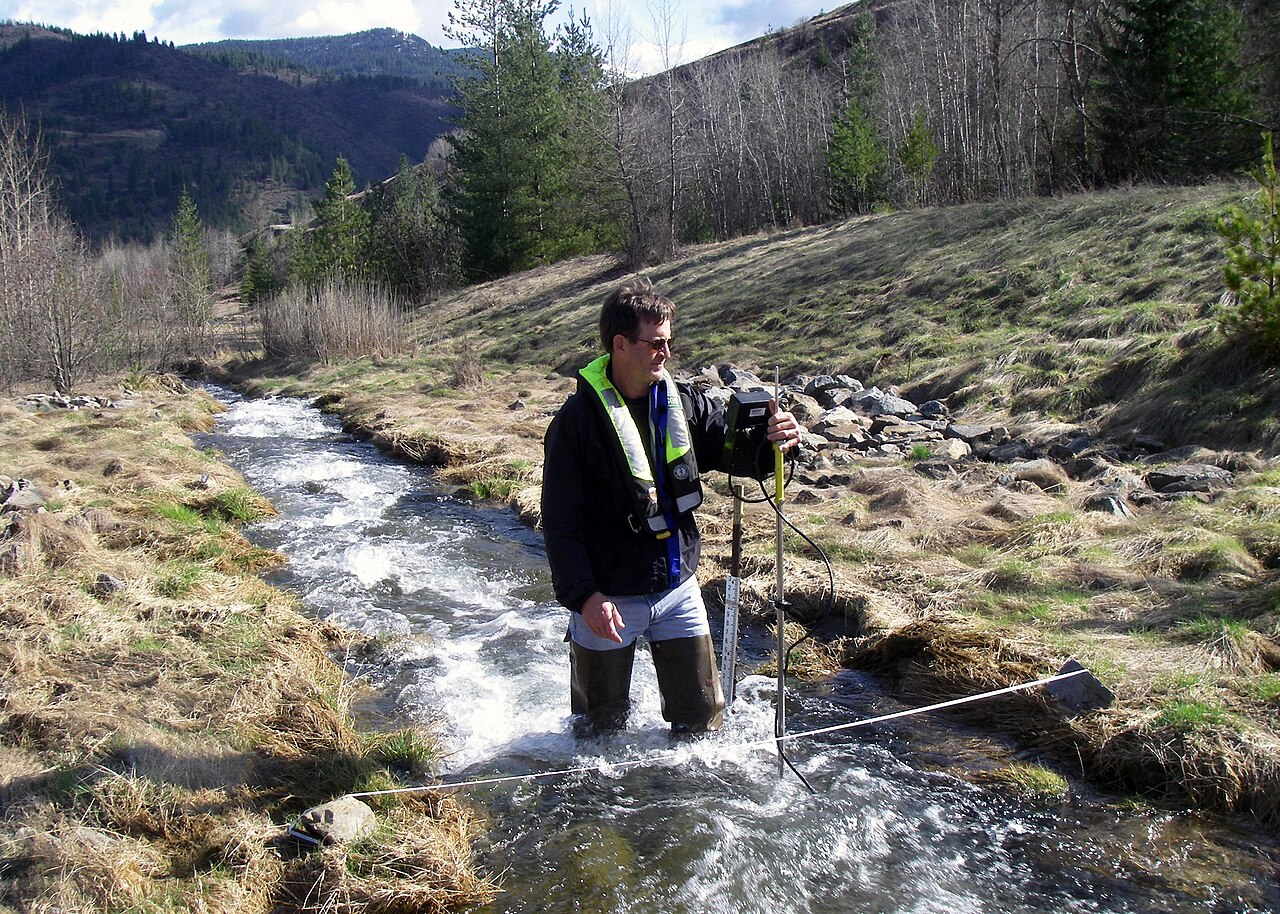
\includegraphics[height=4.6cm]{images/book2/g10-usgs-hydrologist-streamflow.jpg}\hspace{0.3cm}%
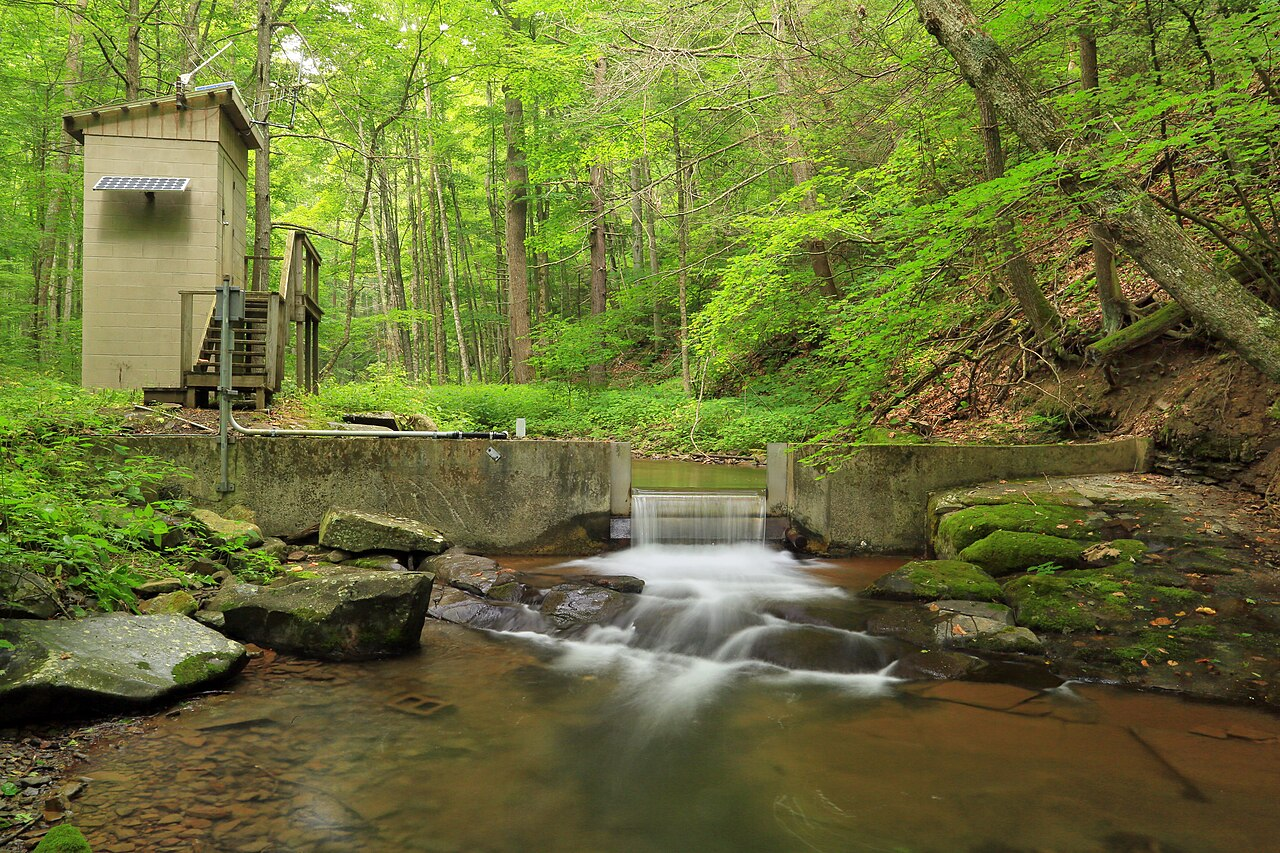
\includegraphics[height=4.6cm]{images/book2/g10-usgs-streamgage.jpg}

{\small बाएँ: एक जलविज्ञानी वेग--क्षेत्रफल विधि से किसी पहाड़ी नाले का \omterm{def:g10:drainage-basins:discharge}{विसर्जन}
मापती है; नाले के आर-पार तना फ़ीता ऊर्ध्वाधरों को
चिह्नित करता है, और छड़ पर एक धारा-मापी लगा है। दाएँ: किसी वन-नाले पर एक प्रवाह-मापन
केंद्र; झोपड़ी में वे उपकरण हैं जो छोटे बाँध के पीछे के जल-तल को
अंकित करते हैं। फ़ोटो: अमेरिकी भूवैज्ञानिक सर्वेक्षण
(सार्वजनिक डोमेन)।}
\end{omfigure}

प्रवाह-मापन में समय लगता है और यह लगातार नहीं किया जा सकता। इसके बजाय प्रवाह-मापन केंद्र
बिना रुके जल के तल को अंकित करता है। अलग-अलग तलों पर किए गए कुछ
प्रवाह-मापन तल और \omterm{def:g10:drainage-basins:discharge}{विसर्जन} को जोड़ने वाला एक वक्र देते हैं,
और केंद्र अपने द्वारा अंकित हर तल को \omterm{def:g10:drainage-basins:discharge}{विसर्जन} में बदल देता है।

बड़ी नदियाँ विशाल \omterm{def:g10:drainage-basins:discharge}{विसर्जन} ले जाती हैं। 1972 से 2003 तक अमेज़न ने
अटलांटिक महासागर को औसतन लगभग \qty{206000}{m^3/s} दिए, लगभग
\qty{6}{\percent} की अनिश्चितता के साथ: यह संसार की नदियों द्वारा समुद्र तक लाए जाने वाले सारे मीठे जल का
लगभग \qty{17}{\percent} है। मिसिसिपी मेक्सिको की खाड़ी तक औसतन
\num{593000} घन फ़ुट प्रति सेकंड, यानी लगभग \qty{16800}{m^3/s}, लाती है:
अमेज़न लगभग बारह गुना अधिक ले जाती है।
% ledger: callede:amazon, kammerer:mississippi

\section{जलालेख}

\begin{definition}[जलालेख; आधार-प्रवाह; विलंब-काल]\label{def:g10:drainage-basins:hydrograph}
\emph{जलालेख}\index{जलालेख} किसी एक बिंदु पर नदी के \omterm{def:g10:drainage-basins:discharge}{विसर्जन} का समय के सापेक्ष
आलेख है। \emph{आधार-प्रवाह}\index{आधार-प्रवाह} \omterm{def:g10:drainage-basins:discharge}{विसर्जन} का वह
भाग है जो भौम जल से पोषित होता है, और जो वर्षाओं के बीच नदी को बहता रखता है। किसी बाढ़ का
\emph{विलंब-काल}\index{विलंब-काल} द्रोणी पर वर्षा के शिखर और \omterm{def:g10:drainage-basins:discharge}{विसर्जन} के शिखर के
बीच का समय है।
\end{definition}

\begin{omfigure}
\begin{tikzpicture}[x=1cm, y=1cm, font=\footnotesize]
  \draw[-{Stealth}] (0,0) -- (10.2,0) node[below left] {समय};
  \draw[-{Stealth}] (0,0) -- (0,5.9) node[above right] {विसर्जन};
  % rain bars hanging from the top
  \draw[black!50] (0,5.4) -- (10,5.4);
  \foreach \x/\h in {1.0/0.15, 1.3/0.35, 1.6/0.55, 1.9/0.4, 2.2/0.2} {
    \fill[omWxRain!70] (\x,5.4) rectangle ++(0.28,-\h);
  }
  \node[anchor=south west] at (2.6,5.4) {द्रोणी पर वर्षा};
  % baseflow and hydrograph
  \fill[omSea] (0,0.7) -- (2.0,0.7) .. controls (2.8,0.8) and (3.3,3.3) .. (4.0,3.6)
    .. controls (4.6,3.6) and (5.1,2.1) .. (6.0,1.55) .. controls (7.0,1.0) and (8.0,0.85) .. (10,0.8)
    -- (10,0) -- (0,0) -- cycle;
  \fill[omLithAlluv] (0,0) -- (0,0.7) -- (2.0,0.7) .. controls (3.5,0.68) and (5.5,0.75) .. (6.6,0.95)
    .. controls (8,1.0) and (9,0.85) .. (10,0.8) -- (10,0) -- cycle;
  \draw[omDef, line width=1.2pt] (0,0.7) -- (2.0,0.7) .. controls (2.8,0.8) and (3.3,3.3) .. (4.0,3.6)
    .. controls (4.6,3.6) and (5.1,2.1) .. (6.0,1.55) .. controls (7.0,1.0) and (8.0,0.85) .. (10,0.8);
  \draw[black!60, dashed] (2.0,0.7) .. controls (3.5,0.68) and (5.5,0.75) .. (6.6,0.95);
  % lag time
  \draw[black!60, densely dotted] (1.74,4.85) -- (1.74,4.3);
  \draw[black!60, densely dotted] (3.98,3.65) -- (3.98,4.3);
  \draw[{Stealth}-{Stealth}] (1.74,4.3) -- node[above] {विलंब-काल} (3.98,4.3);
  % labels
  \node[anchor=west] at (4.2,3.75) {शिखर};
  \node[anchor=east, align=right] at (2.9,2.2) {आरोही\\भुजा};
  \node[anchor=west, align=left] at (5.4,2.3) {अवरोही भुजा};
  \node[align=center] at (4.5,1.25) {अपवाह};
  \node at (8.2,0.4) {आधार-प्रवाह};
\end{tikzpicture}

{\small किसी बाढ़ का \omterm{def:g10:drainage-basins:hydrograph}{जलालेख} (व्यवस्था-चित्र)। वर्षा के बाद \omterm{def:g10:drainage-basins:discharge}{विसर्जन}
एक शिखर तक चढ़ता है और अधिक धीरे वापस गिरता है; वक्र के नीचे का क्षेत्रफल
जल का आयतन है। भौम जल से पोषित \omterm{def:g10:drainage-basins:hydrograph}{आधार-प्रवाह} कम बदलता है; बाक़ी
वह अपवाह है जिसे वर्षा ने जल्दी नदी तक भेज दिया।}
\end{omfigure}

किसी तूफ़ान का जल नदी तक अलग-अलग समय पर पहुँचता है। धारा के पास गिरने वाली
वर्षा मिनटों या घंटों में पहुँचती है; बहुत ऊपर की ओर गिरने वाली वर्षा को
कहीं अधिक समय लगता है, क्योंकि उसे ढलानों से और नदी के अनुदिश बहना पड़ता है।
इसलिए \omterm{def:g10:drainage-basins:discharge}{विसर्जन} \emph{आरोही भुजा} पर तेज़ी से चढ़ता है, जब तक पास की
ढलानों का जल पहुँचता है, तब शिखर पर पहुँचता है जब सबसे अधिक जल एक साथ पहुँचता है, और
\emph{अवरोही भुजा} पर अधिक धीरे गिरता है, जब तक अंतिम जल
द्रोणी के दूर के कोनों से और मृदा से निकलता है। द्रोणी जितनी बड़ी, उतना
लंबा \omterm{def:g10:drainage-basins:hydrograph}{विलंब-काल}: किसी छोटे नाले के लिए घंटे, किसी बड़ी नदी के लिए दिन।

कुछ द्रोणियाँ \emph{आकस्मिक} बाढ़ देती हैं, जिनका शिखर ऊँचा और अचानक और \omterm{def:g10:drainage-basins:hydrograph}{विलंब-काल}
छोटा होता है; दूसरी धीमी, चपटी बाढ़ देती हैं। वही वर्षा अधिक आकस्मिक बाढ़
देती है जब:
\begin{itemize}
  \item द्रोणी छोटी और तीव्र ढलान वाली है, जिससे जल को छोटा, तेज़
        रास्ता तय करना पड़ता है;
  \item ज़मीन थोड़ा ही जल रिसने देती है: नंगी चट्टान, चिकनी मिट्टी, पहले से
        भीगी ज़मीन, जमी हुई ज़मीन, और सबसे बढ़कर किसी नगर की छतें, सड़कें और
        पार्किंग, जो लगभग सारी वर्षा सीधे नालियों
        और नालों में भेज देती हैं;
  \item द्रोणी में नालों और नालियों का घना जाल है, जो
        जल को जल्दी एकत्र करता है।
\end{itemize}
वन, गहरी पारगम्य मृदाएँ और चौड़े बाढ़ के मैदान इसका उलटा करते हैं: वे
जल को रोककर धीरे-धीरे छोड़ते हैं, जिससे शिखर नीचा होता है और देर से आता है।

\subsection*{एक वास्तविक बाढ़}

पोटोमैक नदी पूर्वी संयुक्त राज्य अमेरिका में वॉशिंगटन के पास एक प्रवाह-मापन केंद्र से
ऊपर की ओर \num{11560} वर्ग मील, यानी लगभग
\qty{29900}{km^2}, की द्रोणी का अपवाह करती है। जनवरी 1996 में केंद्र ने
नीचे दिया गया \omterm{def:g10:drainage-basins:hydrograph}{जलालेख} अंकित किया।
% ledger: data:b2-usgs-potomac

\begin{omfigure}
\begin{tikzpicture}
\begin{axis}[omrecord, width=0.86\linewidth, height=6cm, xmin=0, xmax=55, ymin=0, ymax=10000,
  xtick={0,10,20,30,40,50}, xticklabels={5 जनवरी, 15 जनवरी, 25 जनवरी, 4 फ़रवरी, 14 फ़रवरी, 24 फ़रवरी},
  ylabel={विसर्जन (\unit{m^3/s})}, xlabel={1996},
  tick label style={font=\small}, label style={font=\small},
  scaled y ticks=false, yticklabel style={/pgf/number format/fixed}]
\addplot[omDef, line width=1.1pt, mark=*, mark size=1.1pt] table[x=day, y=q] {figdata/out/grade-10-flood_frequency-hydrograph.dat};
\node[anchor=west, font=\footnotesize] at (axis cs:17,9231) {21 जनवरी को \qty{9231}{m^3/s}};
\draw[black!60, dashed] (axis cs:5,334) -- (axis cs:13,334);
\node[anchor=south, font=\footnotesize] at (axis cs:9,1000) {लगभग \qty{330}{m^3/s}};
\draw[black!60] (axis cs:9,1000) -- (axis cs:9,390);
\end{axis}
\end{tikzpicture}

{\small 5 जनवरी से 29 फ़रवरी 1996 तक वॉशिंगटन के पास पोटोमैक नदी का दैनिक माध्य
\omterm{def:g10:drainage-basins:discharge}{विसर्जन}: बाढ़ 18 जनवरी के \qty{362}{m^3/s} से
तीन दिन बाद \qty{9000}{m^3/s} से अधिक तक चढ़ी, फिर आगे के
हफ़्तों में वापस गिरी, जनवरी के अंत में एक छोटे दूसरे उभार के साथ। आँकड़े: अमेरिकी
भूवैज्ञानिक सर्वेक्षण, केंद्र 01646500।}
\end{omfigure}
% values computed in figdata/grade-10/flood_frequency.py (hydro_peak_m3s 9231, hydro_before_mean 334)

बाढ़ से पहले के दिनों में नदी लगभग \qty{330}{m^3/s} ले जा रही थी, जो उसका
\omterm{def:g10:drainage-basins:hydrograph}{आधार-प्रवाह} है। 21 जनवरी को दैनिक माध्य \qty{9231}{m^3/s} तक पहुँचा, लगभग
तीस गुना अधिक। पूरी द्रोणी पर फैलाने पर, उस दिन केंद्र से गुज़रने वाला
जल एक परत बनाता जिसकी मोटाई
$9231 \times 86400 / (29\,900 \times 10^6) \approx \qty{0.027}{m}$, यानी लगभग
\qty{27}{mm} होती: भारी वर्षा जितनी, जो एक ही दिन में पूरी
द्रोणी से एक साथ पहुँचाई गई।
% ledger: data:b2-usgs-potomac (hydro_peak_mm_per_day 26.6 in figdata/grade-10/flood_frequency.py)

\section{बाढ़ और उनका पुनरावृत्ति काल}

किसी नगर को कितनी बड़ी बाढ़ की अपेक्षा करनी चाहिए? उत्तर अतीत से आता है: दशकों से
चल रहा कोई प्रवाह-मापन केंद्र हर वर्ष का सबसे बड़ा \omterm{def:g10:drainage-basins:discharge}{विसर्जन}, यानी
\emph{वार्षिक शिखर}, अंकित कर चुका है। छोटे शिखर लगभग हर वर्ष आते हैं,
बड़े विरले ही। बाढ़ जितनी विरल होती है, उतनी ही बड़ी होती है।

\begin{definition}[पुनरावृत्ति काल]\label{def:g10:drainage-basins:return-period}
किसी बाढ़ का \emph{पुनरावृत्ति काल}\index{पुनरावृत्ति काल} $T$ उन वर्षों के बीच का
औसत अंतराल, वर्षों में, है जिनका वार्षिक शिखर उसके बराबर या उससे अधिक होता है।
पुनरावृत्ति काल $T$ वाली बाढ़, यानी \emph{$T$-वर्षीय बाढ़}, के किसी भी एक वर्ष में बराबर होने या
पार होने की प्रायिकता $1/T$ है।
\end{definition}

सौ-वर्षीय बाढ़ ऐसी बाढ़ नहीं है जो हर सौ वर्ष में एक बार, किसी समय-सारणी की तरह,
आती है। यह ऐसी बाढ़ है जिसके हर वर्ष, हर वर्ष, बराबर होने या पार होने की
संभावना सौ में एक है, चाहे पिछले वर्ष कुछ भी हुआ हो। दो बाढ़ें
लगातार वर्षों में आ सकती हैं; एक शताब्दी बिना एक भी बाढ़ के बीत सकती है।

\begin{method}[वार्षिक शिखरों के अभिलेख से पुनरावृत्ति काल]\label{met:g10:drainage-basins:return-periods}
\begin{enumerate}
  \item $n$ वर्षों के वार्षिक शिखरों की सूची बनाइए।
  \item उन्हें सबसे बड़े (क्रम $m = 1$) से सबसे छोटे
        (क्रम $m = n$) तक क्रम दीजिए।
  \item क्रम $m$ के शिखर को \omterm{def:g10:drainage-basins:return-period}{पुनरावृत्ति काल} $T = (n + 1)/m$ दीजिए।
  \item शिखरों को $T$ के सापेक्ष, $T$ के लघुगणकीय पैमाने पर, आलेखित कीजिए, और
        वांछित \omterm{def:g10:drainage-basins:return-period}{पुनरावृत्ति काल} के लिए \omterm{def:g10:drainage-basins:discharge}{विसर्जन} पढ़िए।
\end{enumerate}
\end{method}

इस प्रकार $n$ शिखरों में सबसे बड़े को $T = n + 1$ वर्ष मिलते हैं:
\num{95} वर्षों के अभिलेख में \num{96} वर्ष। सूत्र वही दर्शाता है जो अभिलेख दिखाता है:
क्रम $m$ का शिखर $m$ वर्षों में बराबर हुआ है या पार हुआ है, कुल $n$ वर्षों में से,
यानी लगभग हर $n/m$ वर्षों में एक बार। यह विधि अभिलेख की लंबाई से आगे भरोसे से
नहीं पहुँच सकती: \num{50} वर्षों का अभिलेख
\num{1000}-वर्षीय बाढ़ के बारे में बहुत कम बताता है।

\begin{omfigure}
\begin{tikzpicture}
\begin{axis}[omrecord, width=0.86\linewidth, height=6.2cm, xmode=log, xmin=0.9, xmax=150,
  ymin=0, ymax=15000, xlabel={पुनरावृत्ति काल $T$ (वर्ष)}, ylabel={वार्षिक शिखर (\unit{m^3/s})},
  xtick={1,2,5,10,20,50,100}, xticklabels={1,2,5,10,20,50,100},
  tick label style={font=\small}, label style={font=\small},
  scaled y ticks=false, yticklabel style={/pgf/number format/fixed}]
\addplot[only marks, mark=*, mark size=1.5pt, omDef] table[x=T, y=peak] {figdata/out/grade-10-flood_frequency-ranked.dat};
\node[anchor=east, font=\footnotesize] at (axis cs:92,13705) {1936};
\node[anchor=east, font=\footnotesize] at (axis cs:46,12658) {1942};
\node[anchor=south, font=\footnotesize] at (axis cs:32,10300) {1972};
\node[anchor=north west, font=\footnotesize, align=left] at (axis cs:1.1,14000) {वॉशिंगटन के पास पोटोमैक नदी,\\वार्षिक शिखर 1931--2025 ($n = 95$)};
\end{axis}
\end{tikzpicture}

{\small वॉशिंगटन के पास पोटोमैक नदी के \num{95} वार्षिक शिखर, क्रम दिए गए
और अपने \omterm{def:g10:drainage-basins:return-period}{पुनरावृत्ति कालों} $T = (n+1)/m$ के सापेक्ष आलेखित। सबसे बड़ा, मार्च
1936 का, $T = 96$ वर्ष पाता है। आँकड़े: अमेरिकी भूवैज्ञानिक सर्वेक्षण, केंद्र 01646500।}
\end{omfigure}
% values computed in figdata/grade-10/flood_frequency.py

\begin{dated}{2026}
वॉशिंगटन के पास पोटोमैक के 1931 से 2025 तक के अभिलेख में पाँच
सबसे बड़े वार्षिक शिखर मार्च 1936 (\qty{13700}{m^3/s}), अक्टूबर 1942,
जून 1972, अप्रैल 1937 और जनवरी 1996 में आए, अंतिम दो बराबर,
\qty{9830}{m^3/s}।
% ledger: data:b2-usgs-potomac
\end{dated}

\subsection*{अनेक वर्षों में बाढ़ की संभावना}

कोई घर या पुल दशकों तक खड़ा रहता है। उसके लिए किसी एक वर्ष में बाढ़ की संभावना
मायने नहीं रखती, बल्कि उसके पूरे जीवनकाल में।

\begin{proposition}[$N$ वर्षों में कम से कम एक बाढ़]\label{prop:g10:drainage-basins:chance}
यदि वर्ष एक-दूसरे से स्वतंत्र हों, तो इसकी प्रायिकता कि
\omterm{def:g10:drainage-basins:return-period}{पुनरावृत्ति काल} $T$ वाली बाढ़ $N$ वर्षों में कम से कम एक बार बराबर हो या पार हो, यह है:
\[
P = 1 - \left(1 - \frac{1}{T}\right)^{N}.
\]
\end{proposition}

\begin{proof}
एक वर्ष में इसकी प्रायिकता कि बाढ़ \emph{नहीं} आती,
$1 - 1/T$ है। वर्षों के स्वतंत्र होने से, इसकी प्रायिकता कि वह $N$ वर्षों में से
किसी में भी नहीं आती, ऐसे $N$ गुणकों का गुणनफल है, $(1 - 1/T)^N$। घटना
``कम से कम एक बार'' ``कभी नहीं'' की विपरीत है, इसलिए उसकी प्रायिकता
$1 - (1 - 1/T)^N$ है।
\end{proof}

तीस वर्षों में सौ-वर्षीय बाढ़ के लिए $(0.99)^{30} \approx 0.740$, और
$P \approx 0.26$: चार में एक संभावना। सौ वर्षों में $(0.99)^{100}
\approx 0.366$ और $P \approx 0.63$: सौ-वर्षीय बाढ़ का सौ वर्षों में आना
निश्चित होने से बहुत दूर है।

\begin{omfigure}
\begin{tikzpicture}
\begin{axis}[omrecord, width=0.82\linewidth, height=5.8cm, xmin=0, xmax=100, ymin=0, ymax=1,
  xlabel={वर्षों की संख्या $N$}, ylabel={कम से कम एक बाढ़ की संभावना},
  ytick={0,0.2,0.4,0.6,0.8,1}, yticklabels={0, 20\,\%, 40\,\%, 60\,\%, 80\,\%, 100\,\%},
  tick label style={font=\small}, label style={font=\small},
  legend pos=south east, legend style={font=\footnotesize}]
\addplot[omThm, line width=1pt] table[x=n, y=p10] {figdata/out/grade-10-flood_frequency-chance.dat};
\addplot[omProp, line width=1pt] table[x=n, y=p50] {figdata/out/grade-10-flood_frequency-chance.dat};
\addplot[omDef, line width=1pt] table[x=n, y=p100] {figdata/out/grade-10-flood_frequency-chance.dat};
\legend{{10-वर्षीय बाढ़}, {50-वर्षीय बाढ़}, {100-वर्षीय बाढ़}}
\draw[black!60, dashed] (axis cs:30,0) -- (axis cs:30,0.2603) -- (axis cs:0,0.2603);
\fill[omDef] (axis cs:30,0.2603) circle (2pt);
\node[anchor=north west, font=\footnotesize] at (axis cs:31,0.22) {30 वर्षों में 26\,\%};
\end{axis}
\end{tikzpicture}

{\small इसकी संभावना कि 10, 50 या 100 वर्ष \omterm{def:g10:drainage-basins:return-period}{पुनरावृत्ति काल} वाली बाढ़ $N$ वर्षों में
कम से कम एक बार आए।}
\end{omfigure}
% values computed in figdata/grade-10/flood_frequency.py (chance_100_30 0.2603)

\section{बाँध और तटबंध}

लोगों ने बहुत पहले से ऐसी संरचनाएँ बनाई हैं जो बाढ़ के गुज़रने का ढंग बदल देती हैं। दो संरचनाएँ
इसे उलटे ढंगों से बदलती हैं।

\emph{बाँध} एक जलाशय को रोके रखता है। जब बाढ़ आती है, तो उसके जल का एक भाग
जलाशय में संचित होता है, जिसका तल चढ़ जाता है, और बाद में,
अधिक लंबे समय में, छोड़ा जाता है। नीचे की ओर जल का उतना ही आयतन गुज़रता है, पर फैलकर:
शिखर नीचा और देर से होता है। जलाशय बाढ़ को केवल तब तक नीचा करता है जब तक
उसमें जगह बची है; भर जाने पर उसमें आने वाला सारा जल आगे निकल जाता है।

\emph{तटबंध} मिट्टी का एक बाँध है जो नदी के अनुदिश बनाया जाता है ताकि उसकी बाढ़ें
बाढ़ के मैदान से दूर रहें। तटबंधों के बीच जल फैल नहीं पाता; उसी
\omterm{def:g10:drainage-basins:discharge}{विसर्जन} को संकरी काट से ले जाने के लिए उसे ऊँचा खड़ा होना और अधिक तेज़ बहना
पड़ता है। तटबंधों के पीछे की भूमि सूखी रहती है, जब तक तटबंध टिके रहें और
उनके ऊपर से जल न बहे। पर बाढ़ के मैदान में अब बाढ़ के दौरान जल संचित नहीं होता,
इसलिए उसका अधिक भाग, और अधिक जल्दी, नीचे की ओर जाता है।

\begin{omfigure}
\begin{tikzpicture}[x=0.62cm, y=0.62cm, font=\footnotesize]
  \begin{scope}
    \draw[-{Stealth}] (0,0) -- (9.4,0) node[below left] {समय};
    \draw[-{Stealth}] (0,0) -- (0,6.0) node[above right] {विसर्जन};
    \draw[omDef, line width=1.2pt] (0,0.6) -- (1,0.6) .. controls (1.8,0.7) and (2.2,5.2) .. (2.8,5.2)
      .. controls (3.5,5.2) and (4,1.6) .. (5,1.0) .. controls (6,0.7) and (7.5,0.6) .. (9,0.6);
    \draw[omThm, line width=1.2pt, dashed] (0,0.6) -- (1.3,0.6) .. controls (2.3,0.75) and (3.0,3.3) .. (3.8,3.3)
      .. controls (4.7,3.3) and (5.8,1.5) .. (6.8,1.0) .. controls (7.6,0.75) and (8.3,0.65) .. (9,0.6);
    \node[anchor=west, text=omDef] at (3.0,5.35) {जलाशय में आता};
    \node[anchor=west, text=omThm] at (4.2,3.55) {बाँध के नीचे};
    \node[anchor=north] at (4.5,-0.45) {(a) बाँध: नीचा, देर से शिखर};
  \end{scope}
  \begin{scope}[xshift=7.2cm]
    \fill[omLithAlluv] (0,0) -- (10,0) -- (10,1.8) -- (0,1.8) -- cycle;
    \fill[white] (3.5,1.8) -- (3.9,0.4) -- (6.1,0.4) -- (6.5,1.8) -- cycle;
    \fill[omSea] (0.4,2.3) -- (3.25,2.3) -- (3.5,1.8) -- (3.9,0.4) -- (6.1,0.4) -- (6.5,1.8) -- (6.75,2.3) -- (9.6,2.3) -- (9.6,1.8) -- (0.4,1.8) -- cycle;
    \draw[line width=0.8pt, brown!60!black] (0,1.8) -- (3.5,1.8) -- (3.9,0.4) -- (6.1,0.4) -- (6.5,1.8) -- (10,1.8);
    \draw[omDef!70!black] (0.4,2.3) -- (9.6,2.3);
    \node[anchor=south, text=omDef!70!black, align=center] at (1.5,2.35) {तटबंधों\\के बिना};
    % levees
    \fill[brown!45] (2.6,1.8) -- (3.0,3.9) -- (3.3,3.9) -- (3.5,1.8) -- cycle;
    \fill[brown!45] (6.5,1.8) -- (6.7,3.9) -- (7.0,3.9) -- (7.4,1.8) -- cycle;
    \fill[omSea!70!omDef] (3.5,1.8) -- (3.9,0.4) -- (6.1,0.4) -- (6.5,1.8) -- (6.65,3.4) -- (3.35,3.4) -- cycle;
    \draw[omThm, line width=0.8pt, dashed] (3.35,3.4) -- (6.65,3.4);
    \node[anchor=south, text=omThm] at (5,3.95) {तटबंधों के साथ};
    \draw[omThm] (5,3.95) -- (5,3.45);
    \node[anchor=north] at (5,-0.45) {(b) तटबंध: बाढ़ ऊँची खड़ी होती है};
  \end{scope}
\end{tikzpicture}

{\small व्यवस्था-चित्र। (a) एक जलाशय बाढ़ का एक भाग संचित करता है और उसे बाद में
छोड़ता है: बाँध के नीचे शिखर नीचा होता है और देर से आता है। (b) तटबंधों के बिना
बाढ़ बाढ़ के मैदान पर पतली परत में फैल जाती है; तटबंधों के बीच वही
\omterm{def:g10:drainage-basins:discharge}{विसर्जन} संकरी काट से गुज़रना पड़ता है और कहीं अधिक ऊँचा खड़ा होता है।}
\end{omfigure}

\section{अभ्यास}

\begin{exercise}[$\star$]\label{exo:g10:drainage-basins:1}
\omterm{def:g10:drainage-basins:drainage-basin}{अपवाह द्रोणी} और \omterm{def:g10:drainage-basins:drainage-basin}{जल-विभाजक} की परिभाषा दीजिए। एक मीटर की दूरी पर गिरने वाली वर्षा की दो बूँदें
दो अलग-अलग समुद्रों में क्यों पहुँच सकती हैं?
\end{exercise}

\begin{exercise}[$\star$]\label{exo:g10:drainage-basins:2}
नदी के \omterm{def:g10:drainage-basins:discharge}{विसर्जन} की परिभाषा दीजिए और उसकी इकाई बताइए। \qty{1}{m^3/s} ले जाने वाली नदी के किसी
बिंदु से एक दिन में कितने लीटर गुज़रते हैं?
\end{exercise}

\begin{exercise}[$\star$]\label{exo:g10:drainage-basins:3}
जनवरी 1996 के पोटोमैक के \omterm{def:g10:drainage-basins:hydrograph}{जलालेख} पर बाढ़ से पहले का \omterm{def:g10:drainage-basins:hydrograph}{आधार-प्रवाह},
शिखर \omterm{def:g10:drainage-basins:discharge}{विसर्जन} और उसकी तिथि, और चढ़ाव में लगे
दिनों की संख्या पढ़िए।
\end{exercise}

\begin{exercise}[$\star$]\label{exo:g10:drainage-basins:4}
इसकी प्रायिकता क्या है कि अगले वर्ष कोई \num{50}-वर्षीय बाढ़ बराबर हो या पार हो?
पिछले वर्ष एक \num{50}-वर्षीय बाढ़ आई थी: क्या इस वर्ष उसकी संभावना कम
है?
\end{exercise}

\begin{exercise}[$\star$]\label{exo:g10:drainage-basins:5}
मिसिसिपी औसतन प्रति सेकंड \num{593000} घन फ़ुट जल
समुद्र तक लाती है (\num{1}~फ़ुट = \qty{0.3048}{m})। इस \omterm{def:g10:drainage-basins:discharge}{विसर्जन} को
\unit{m^3/s} में बदलिए, और इसकी तुलना अमेज़न के \qty{206000}{m^3/s} से
कीजिए।
\end{exercise}

\begin{exercise}[$\star\star$]\label{exo:g10:drainage-basins:6}
एक जलविज्ञानी \qty{1.5}{m} की दूरी पर चार ऊर्ध्वाधरों से एक धारा का प्रवाह-मापन करता है।
गहराइयाँ \num{0.3}, \num{0.6}, \num{0.7} और \qty{0.4}{m} हैं; माध्य
वेग \num{0.2}, \num{0.5}, \num{0.6} और \qty{0.3}{m/s}। अनुप्रस्थ
काट, \omterm{def:g10:drainage-basins:discharge}{विसर्जन} और माध्य वेग परिकलित कीजिए।
\end{exercise}

\begin{exercise}[$\star\star$]\label{exo:g10:drainage-basins:7}
एक तूफ़ान मानचित्र पर वार्डन नदी की पूरी द्रोणी, \qty{66}{km^2}, पर \qty{20}{mm} वर्षा
करता है। यह जल का कितना आयतन है? यदि यह सारा जल
दो दिनों में निकास तक पहुँचे, तो माध्य अतिरिक्त \omterm{def:g10:drainage-basins:discharge}{विसर्जन} क्या होगा?
\end{exercise}

\begin{exercise}[$\star\star$]\label{exo:g10:drainage-basins:8}
किसी छोटी नदी के नौ वर्षों के वार्षिक शिखर, \unit{m^3/s} में, ये हैं:
\num{42}, \num{65}, \num{38}, \num{120}, \num{51}, \num{47}, \num{88},
\num{35}, \num{59}। इन्हें क्रम दीजिए और तीन सबसे बड़े शिखरों के \omterm{def:g10:drainage-basins:return-period}{पुनरावृत्ति काल} बताइए।
माध्यिका शिखर का \omterm{def:g10:drainage-basins:return-period}{पुनरावृत्ति काल} क्या है?
\end{exercise}

\begin{exercise}[$\star\star$]\label{exo:g10:drainage-basins:9}
एक ही तूफ़ान समान क्षेत्रफल की दो द्रोणियों पर गिरता है: एक तीव्र ढलान वाली, नगर से ढकी,
दूसरी हल्की ढलान वाली और वनाच्छादित। उनके दोनों \omterm{def:g10:drainage-basins:hydrograph}{जलालेखों} का रेखाचित्र
एक ही अक्षों पर बनाइए और अंतर समझाइए।
\end{exercise}

\begin{exercise}[$\star\star$]\label{exo:g10:drainage-basins:10}
21 जनवरी 1996 के शिखर पर पोटोमैक \qty{29900}{km^2} की
द्रोणी से \qty{9231}{m^3/s} ले जा रही थी। पूरी द्रोणी पर फैलाने पर इस \omterm{def:g10:drainage-basins:discharge}{विसर्जन} का
एक दिन जल की कितनी गहराई दर्शाता है? इसकी तुलना
\qty{330}{m^3/s} के \omterm{def:g10:drainage-basins:hydrograph}{आधार-प्रवाह} से कीजिए।
\end{exercise}

\begin{exercise}[$\star\star$]\label{exo:g10:drainage-basins:11}
इसकी प्रायिकता क्या है कि कोई \num{10}-वर्षीय बाढ़ \num{10} वर्षों में कम से कम एक बार
आए? और इसकी कि वह इन दस वर्षों में बिल्कुल न आए?
\end{exercise}

\begin{exercise}[$\star\star\star$]\label{exo:g10:drainage-basins:12}
बाढ़ के समय किसी जलाशय में आने वाला \omterm{def:g10:drainage-basins:discharge}{विसर्जन} एक दिन में \qty{0}{m^3/s} से
\qty{1200}{m^3/s} तक समान रूप से चढ़ता है, फिर दो दिनों में समान रूप से वापस
\qty{0}{m^3/s} तक गिरता है (\omterm{def:g10:drainage-basins:hydrograph}{आधार-प्रवाह} उपेक्षित)। बाढ़ कितना आयतन
लाती है? बाँध अधिकतम \qty{800}{m^3/s} निकलने देता है, और जलाशय
\num{60} मिलियन \unit{m^3} संचित कर सकता है। क्या वह
\qty{800}{m^3/s} से ऊपर का सब कुछ रोक सकता है?
\end{exercise}

\begin{exercise}[$\star\star\star$]\label{exo:g10:drainage-basins:13}
\qty{100}{m} चौड़ी एक नदी \qty{800}{m^3/s} पर अपने किनारों तक भरी है, और
\qty{2}{m/s} से बहती है। \qty{1200}{m^3/s} की बाढ़ आती है।
\begin{enumerate}
  \item तटबंधों के बिना अतिरिक्त \qty{400}{m^3/s} \qty{900}{m} चौड़े
        बाढ़ के मैदान पर फैल जाता है, जहाँ वह \qty{0.5}{m/s} से बहता है। बाढ़ के मैदान पर
        जल कितना गहरा है?
  \item तटबंधों के साथ सारी बाढ़ उनके बीच से, \qty{2}{m/s} से, गुज़रती है।
        नदी कितनी गहरी है, और वह अपने किनारों से कितनी ऊपर खड़ी है?
\end{enumerate}
\end{exercise}

\begin{exercise}[$\star\star\star$]\label{exo:g10:drainage-basins:14}
कौन-सा \omterm{def:g10:drainage-basins:return-period}{पुनरावृत्ति काल} $T$ किसी बाढ़ को \num{30} वर्षों में कम से कम एक बार आने की
दो में एक संभावना देता है?
\end{exercise}

\begin{exercise}[$\star\star\star$]\label{exo:g10:drainage-basins:15}
एक छोटे मानचित्र को \qty{100}{m} के वर्गों में काटा गया है; मीटर में उनकी ऊँचाइयाँ
नीचे दी गई हैं (उत्तर ऊपर)। जल हर वर्ग से उसके चार पड़ोसियों
(उत्तर, दक्षिण, पूर्व, पश्चिम) में से सबसे निचले की ओर निकलता है, यदि वह निचला है; \qty{34}{m} (उत्तर-पश्चिमी कोना) और \qty{30}{m} (दक्षिण-पूर्वी कोना) वाले वर्ग
दो नालों के
निकास हैं।
\begin{center}
\begin{tabular}{|c|c|c|c|}
\hline
34 & 38 & 46 & 50 \\ \hline
37 & 42 & 48 & 47 \\ \hline
45 & 49 & 44 & 39 \\ \hline
51 & 46 & 37 & 30 \\ \hline
\end{tabular}
\end{center}
हर वर्ग की प्रवाह-दिशा बनाइए, हर निकास की द्रोणी और
उसका क्षेत्रफल ज्ञात कीजिए, और \omterm{def:g10:drainage-basins:drainage-basin}{जल-विभाजक} बनाइए।
\end{exercise}

\section{समस्या: सौ-वर्षीय बाढ़}

\begin{problem}[{सप्ताहांत समस्या --- नदी कितनी बार नगर में आती है?}]
\label{pb:g10:drainage-basins:1}
% ledger: data:b2-usgs-potomac (values computed in figdata/grade-10/flood_frequency.py)
वॉशिंगटन से ठीक ऊपर की ओर, पोटोमैक नदी पर बसे एक नगर की कल्पना कीजिए, जिसके पास एक
प्रवाह-मापन केंद्र है जिसने 1931 से हर वर्ष नदी का सबसे बड़ा \omterm{def:g10:drainage-basins:discharge}{विसर्जन} अंकित किया
है। वार्षिक शिखर नीचे बनाए गए हैं; जनवरी 1996 का
\omterm{def:g10:drainage-basins:hydrograph}{जलालेख} अध्याय में दिया गया है।

\begin{center}
\begin{tikzpicture}
\begin{axis}[omrecord, width=0.9\linewidth, height=5.4cm, ybar, bar width=1.6pt, xmin=1929, xmax=2027,
  ymin=0, ymax=15000, ylabel={वार्षिक शिखर (\unit{m^3/s})}, xlabel={वर्ष},
  xtick={1930,1950,1970,1990,2010}, xticklabel style={/pgf/number format/1000 sep={}},
  tick label style={font=\small}, label style={font=\small},
  scaled y ticks=false, yticklabel style={/pgf/number format/fixed}]
\addplot[fill=omDef!70, draw=none] table[x=year, y=peak] {figdata/out/grade-10-flood_frequency-record.dat};
\draw[omThm, dashed] (axis cs:1929,9500) -- (axis cs:2027,9500);
\node[anchor=south east, font=\footnotesize, text=omThm] at (axis cs:2026,9500) {\qty{9500}{m^3/s}};
\end{axis}
\end{tikzpicture}

{\small वॉशिंगटन के पास पोटोमैक नदी के वार्षिक शिखर \omterm{def:g10:drainage-basins:discharge}{विसर्जन}, जल-वर्ष
1931--2025 (जल-वर्ष अक्टूबर से सितंबर तक चलता है: अक्टूबर
1942 की बाढ़ 1943 में गिनी जाती है)। आँकड़े: अमेरिकी भूवैज्ञानिक सर्वेक्षण, केंद्र 01646500।}
\end{center}

\medskip
\noindent\textbf{भाग I --- द्रोणी और विसर्जन।}
\begin{enumerate}
  \item केंद्र की द्रोणी \num{11560} वर्ग मील में फैली है
        (\num{1}~मील = \qty{1.609}{km})। इस क्षेत्रफल को
        \unit{km^2} में बदलिए।
  \item मानचित्र पर कौन-सी रेखा इस क्षेत्र को घेरती है?
  \item सबसे बड़ा शिखर, 19 मार्च 1936 को, \num{484000} घन फ़ुट प्रति
        सेकंड था। इसे \unit{m^3/s} में बदलिए (\num{1}~फ़ुट =
        \qty{0.3048}{m})।
  \item माध्यिका वार्षिक शिखर \qty{3341}{m^3/s} है। 1936 की बाढ़ माध्यिका से
        कितने गुना बड़ी थी?
  \item मान लीजिए कि 1936 के शिखर पर केंद्र के पास नदी \qty{400}{m} चौड़ी और
        औसतन \qty{8}{m} गहरी थी। उसका माध्य
        वेग क्या रहा होगा?
\end{enumerate}

\medskip
\noindent\textbf{भाग II --- 1996 की बाढ़ को पढ़ना।}
\begin{enumerate}[resume]
  \item जनवरी 1996 के \omterm{def:g10:drainage-basins:hydrograph}{जलालेख} पर बाढ़ से पहले के दिनों में
        \omterm{def:g10:drainage-basins:hydrograph}{आधार-प्रवाह} क्या था?
  \item शिखर दैनिक \omterm{def:g10:drainage-basins:discharge}{विसर्जन} क्या था, और किस दिन?
  \item 18 जनवरी के \qty{362}{m^3/s} से शिखर तक
        चढ़ाव में कितने दिन लगे?
  \item शिखर-दिवस ने पूरी द्रोणी पर कितनी गहराई का जल केंद्र
        से आगे पहुँचाया?
  \item एक दूसरा, छोटा उभार 29 जनवरी को शिखर पर पहुँचता है। यह द्रोणी तक पहुँचने वाले
        जल के बारे में क्या बताता है?
  \item 7 फ़रवरी को \omterm{def:g10:drainage-basins:discharge}{विसर्जन} वापस लगभग \qty{410}{m^3/s} पर था। यह शिखर के कितने
        समय बाद था? अवरोही भुजा आरोही भुजा से अधिक
        समय तक क्यों चलती है?
\end{enumerate}

\medskip
\noindent\textbf{भाग III --- बाढ़ों को क्रम देना।}
\begin{enumerate}[resume]
  \item अभिलेख में $n = 95$ वार्षिक शिखर हैं। विधि सबसे बड़े शिखर को कौन-सा
        \omterm{def:g10:drainage-basins:return-period}{पुनरावृत्ति काल} देती है?
  \item अक्टूबर 1942 का शिखर (\qty{12658}{m^3/s}) दूसरे क्रम पर है। उसका
        \omterm{def:g10:drainage-basins:return-period}{पुनरावृत्ति काल} क्या है?
  \item जून 1972 का शिखर (\qty{10166}{m^3/s}) तीसरे क्रम पर है। उसका
        \omterm{def:g10:drainage-basins:return-period}{पुनरावृत्ति काल} क्या है?
  \item अप्रैल 1937 और जनवरी 1996 की बाढ़ें बराबर थीं
        (\qty{9826}{m^3/s})। क्रम 4 और 5 दिए जाने पर उन्हें कौन-से \omterm{def:g10:drainage-basins:return-period}{पुनरावृत्ति काल}
        मिलते हैं? क्या यहाँ एक ही मान साझा करना बहुत मायने रखता है?
  \item दंड आरेख पर उन वर्षों को गिनिए जिनका शिखर
        \qty{9500}{m^3/s} से अधिक था। किसी एक वर्ष में ऐसे शिखर की संभावना
        का, और उसके \omterm{def:g10:drainage-basins:return-period}{पुनरावृत्ति काल} का, अनुमान लगाइए।
\end{enumerate}

\medskip
\noindent\textbf{भाग IV --- बाढ़ की संभावना।}
\begin{enumerate}[resume]
  \item इसकी प्रायिकता क्या है कि किसी दिए हुए वर्ष में कोई \num{100}-वर्षीय बाढ़ बराबर हो या
        पार हो?
  \item इसकी प्रायिकता क्या है कि उस वर्ष ऐसा न हो?
  \item इसकी प्रायिकता क्या है कि वह \num{30} वर्षों में न आए,
        यानी उतने समय में जितना कोई परिवार नदी के किनारे के घर में रह सकता है?
  \item \num{30} वर्षों में कम से कम एक \num{100}-वर्षीय बाढ़ की संभावना
        क्या है?
\end{enumerate}
\end{problem}
